\documentclass{../../zirkelblatt1415}
\usepackage{mathtools}
\usepackage{booktabs}
\usepackage{relsize}
\let\raggedsection\centering

\usepackage[T1]{fontenc}
\usepackage{libertine}

\usepackage[cmtip,all]{xy}
\newcommand{\longsquiggly}{\!\!\xymatrix{{}\ar@{~>}[r]&{}}\!\!}

\newcommand{\cell}[1]{\framebox{#1}}
\newcommand{\blank}{\phantom{0}}

\renewcommand*\theenumi{\arabic{enumi}}
\renewcommand{\labelenumi}{\theenumi.}

\begin{document}

\begin{center}
  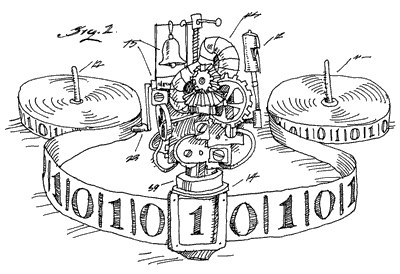
\includegraphics[scale=0.5]{turing-machine}
\end{center}

\section*{Spiel und Spaß mit Turingmaschinen}

\begin{enumerate}
\item Entwerfe eine Turingmaschine, die abwechselnd Nullen und Eisen aufs Band
schreibt.

\emph{Beispiel:} \cell{\blank} $\longsquiggly$
\cell{0}\cell{1}\cell{0}\cell{1}\cell{0}\cell{1}$\cdots$

\item Entwerfe eine Turingmaschine, die eine~$0$ vor die gesamte Eingabe setzt
und dabei die Eingabe nach rechts verschiebt.

\emph{Beispiel:} \cell{1}\cell{0}\cell{1}\cell{1}\cell{\blank} $\longsquiggly$
\cell{0}\cell{1}\cell{0}\cell{1}\cell{1}\cell{\blank}

\item Entwerfe eine Turingmaschine, die eine gegebene natürliche Zahl um Eins
erhöht. Die Eingabe erfolgt als Binärdarstellung (mit den Einern vorne, den
Zweiern an zweiter Stelle, den Vierern dahinter -- also genau umgekehrt als in
der üblichen Notation).

\emph{Beispiele:}
\cell{0}\cell{1}\cell{1}\cell{\blank} $\longsquiggly$
\cell{1}\cell{1}\cell{1}\cell{\blank},\quad
\cell{1}\cell{1}\cell{1}\cell{\blank} $\longsquiggly$
\cell{0}\cell{0}\cell{0}\cell{1}\cell{\blank}

\emph{Bonusaufgabe:} Schreibe die Maschine so um, dass Ein- und Ausgabe in der
gewohnten Schreib- und Leserichtung erfolgen (also mit den Einern ganz rechts
statt ganz links). Beachte, dass die Turingmaschine trotzdem am linken Ende
startet!

\item Entwerfe eine Turingmaschine, die die Eingabe vollständig kopiert.

\emph{Beispiel:} \cell{1}\cell{0}\cell{1}\cell{\blank} $\longsquiggly$
\cell{1}\cell{0}\cell{1}\cell{\blank}\cell{1}\cell{0}\cell{1}\cell{\blank}

\item Entwerfe eine Turingmaschine, die prüft, ob die Eingabe ein Palindrom ist
(zum Beispiel ist~"`0010100"' ein Palindrom, aber~"`0010110"' nicht).
Meinetwegen darf dabei die Eingabe zerstört werden. Die Maschine soll je
nachdem, ob die Eingabe ein Palindrom ist, in einem anderen Zustand halten.

\item Entwerfe eine Turingmaschine, die eine Eins, dann zwei Einsen, dann drei
Einsen, und so weiter aufs Band schreibt.

\emph{Beispiel:} \cell{\blank} $\longsquiggly$
\cell{1}\cell{\blank}\cell{1}\cell{1}\cell{\blank}\cell{1}\cell{1}\cell{1}\cell{\blank}\cell{1}\cell{1}\cell{1}\cell{1}\cell{\blank}\cell{1}\cell{1}\cell{1}\cell{1}\cell{1}\cell{\blank}$\cdots$

\item Entwerfe eine Turingmaschine, die vergleicht, ob zwei Ziffernfolgen
gleich sind oder nicht. Sie soll in verschiedenen Zuständen halten, je nachdem,
ob die Folgen gleich sind oder nicht.

\emph{Beispiel:} Bei Eingabe von
\cell{0}\cell{1}\cell{1}\cell{0}\cell{\blank}\cell{0}\cell{1}\cell{0}\cell{0}\cell{\blank}
soll die Turingmaschine in einem anderen Zustand halten als bei
\cell{0}\cell{1}\cell{1}\cell{0}\cell{\blank}\cell{0}\cell{1}\cell{0}\cell{1}\cell{\blank}.

\item Entwerfe eine Turingmaschine, die zwei in Binärdarstellung gegebene
Zahlen addiert.

\emph{Beispiele:}
\cell{1}\cell{0}\cell{1}\cell{\blank}\cell{0}\cell{1}\cell{1}\cell{1}\cell{\blank}
$\longsquiggly$
\cell{1}\cell{1}\cell{0}\cell{0}\cell{1}\cell{\blank}

\item Entwerfe eine Turingmaschine, die das gesamte Band (nach rechts hin) mit
Nullen und Einsen vollschreibt: Und zwar soll an die~$n$-te Position genau dann
eine Eins geschrieben werden, wenn~$n$ eine Primzahl ist.

\emph{Beispiel:}
\cell{\blank} $\longsquiggly$
\cell{0}\cell{1}\cell{1}\cell{0}\cell{1}\cell{0}\cell{1}\cell{0}\cell{0}\cell{0}\cell{1}\cell{0}\cell{1}\cell{0}\cell{0}\cell{0}\cell{1}\cell{0}$\cdots$

\item Es macht keinen wesentlichen Unterschied, ob das Band in beide Richtungen
beliebig lang ist oder nur nach rechts. Um das einzusehen, erkläre wie man aus
einer Turingmaschine, die ein beidseitig unbeschränktes Band erwartet, eine
Maschine basteln kann, die auch auf einem nur nach rechts beliebig langen Band
funktioniert.

\end{enumerate}

\end{document}
